%%
%% CSE 8673 (Machine Learning), Fall 2026, Mississippi State University
%% Term paper: 8-page conference draft, double column (ACM sigconf).
%% Overleaf project name: AditPatel_BiomedicalML_CSE_8673
%%
%% Phase 0 set the title and abstract. Phase 1 added the literature survey
%% and the paper list in literature_list.csv. Phase 2 reorganized the paper
%% to follow the course template (TERM_PAPER_TEMPLATE_DATAPOINTS): research
%% challenges, proposed methodology, experimental methodology, planned
%% results, the six-week plan, and the two required sections at the end.
%% The Phase 1 version is in Overleaf's history.
%%
%% Compile with pdfLaTeX + BibTeX (Overleaf default).
%% "nonacm" removes the ACM copyright block and reference-format box,
%% since this is a course paper and not an ACM submission.
%%
\documentclass[sigconf,nonacm]{acmart}

\AtBeginDocument{%
  \providecommand\BibTeX{{%
    Bib\TeX}}}

\usepackage{amsmath}
\usepackage{booktabs}
%% Figure 1 is drawn with plain TikZ instead of the forest package, because
%% forest was too slow for Overleaf's 10-second free compile limit.
\usepackage{tikz}
\usetikzlibrary{arrows.meta,calc,fit,positioning}
\usepackage{tabularx}

%% Left-aligned table columns. P{width} has a fixed width and L stretches.
\newcolumntype{P}[1]{>{\raggedright\arraybackslash}p{#1}}
\newcolumntype{L}{>{\raggedright\arraybackslash}X}

%% Let a column end short instead of stretching the space between blocks.
\raggedbottom

%% Page numbers, so page counts are easy to check.
\settopmatter{printfolios=true}

\begin{document}

\title{Group-Robust Shift-Aware Temperature Scaling for Adapted Medical
  Foundation Models Under Image Corruption}

\author{Adit Patel}
\affiliation{%
  \institution{Mississippi State University}
  \department{Department of Computer Science and Engineering}
  \city{Mississippi State}
  \state{Mississippi}
  \country{USA}}
  \email{adp543@msstate.edu}

\renewcommand{\shortauthors}{Patel}

\begin{abstract}
Medical foundation models are usually adapted by linear probing or LoRA
and calibrated with temperature scaling on clean validation images. Real
test images are often noisy, blurry, or badly lit, and a calibrator fit on
clean data can then give overconfident risks, possibly more so for some
patient groups, which could mislead biopsy decisions. Shift-aware
calibrators target only average calibration, and group-aware ones assume
test data look like calibration data. I propose Group-Robust Shift-Aware
Temperature Scaling (GR-SATS), a post-hoc calibrator that sets a per-image
temperature from a standardized nearest-neighbor shift score and fits its
two parameters for the worst-off patient group. The fit is convex and needs
group labels only while fitting. I will evaluate it on HAM10000 (sex and
age groups) and Fitzpatrick17k (skin-type groups) with DINOv2 and
BiomedCLIP adapted by linear probing and LoRA, on MedMNIST-C corruption
families held out from fitting, at five severities. Baselines include
temperature scaling variants, density-aware calibration,
atypicality-aware recalibration, and cluster-wise temperature scaling, and
the main metrics are worst-group negative log-likelihood and Brier score. The expected
contribution is, as far as I know, the first worst-group, shift-aware
post-hoc calibrator for medical imaging, plus a measurement of how subgroup
calibration degrades under corruption.
\end{abstract}

\begin{CCSXML}
<ccs2012>
 <concept>
  <concept_id>10010147.10010257</concept_id>
  <concept_desc>Computing methodologies~Machine learning</concept_desc>
  <concept_significance>500</concept_significance>
 </concept>
 <concept>
  <concept_id>10010405.10010444</concept_id>
  <concept_desc>Applied computing~Life and medical sciences</concept_desc>
  <concept_significance>300</concept_significance>
 </concept>
</ccs2012>
\end{CCSXML}

\ccsdesc[500]{Computing methodologies~Machine learning}
\ccsdesc[300]{Applied computing~Life and medical sciences}

\keywords{calibration, temperature scaling, distribution shift, image
  corruption, fairness, subgroup robustness, medical foundation models}

\maketitle

%% =========================================================
\section{Introduction}
\label{sec:intro}

Foundation models pretrained on large image collections are now a common starting point for medical image classification \cite{moor2023generalist,oquab2024dinov2,zhang2025biomedclip}. They are usually adapted by training a linear head on frozen features, called linear probing (LP), or by fine-tuning a small set of added low-rank weights with LoRA \cite{hu2022lora,jin2024fairmedfm}. In dermatology, an adapted model might estimate the probability that a lesion is malignant, and a clinician might use that number to decide whether to biopsy. This only works if the probabilities are calibrated, so that about 20\% of the lesions given a 20\% risk are actually malignant \cite{guo2017calibration}.

Calibration is usually checked on clean validation images, but real images vary in quality. Clinical photos can be blurry, compressed, or badly lit, and dermoscopy images can have black corners or text overlays \cite{disalvo2024medmnistc}. Calibration gets worse as images move away from the training distribution \cite{ovadia2019trust}, and post-hoc calibrators fit on clean data become overconfident under this kind of shift \cite{tomani2021posthoc}. Calibration also differs between patient groups. Leading skin cancer models were miscalibrated across sex, skin tone, and age on new datasets \cite{dominique2025calibration}, and a skin condition classifier was most accurate on skin types similar to the ones it was trained on \cite{groh2021fitzpatrick}. The groups most at risk also tend to be the smallest. In the cleaned Fitzpatrick17k \cite{abhishek2025quality}, skin types V and VI make up 11\% of the images with a known skin type, and its validation and test sets together hold only 32 cancers from these types.

Shift-aware calibrators such as density-aware calibration (DAC) keep average calibration under shift \cite{tomani2021posthoc,yu2022multidomain,tomani2023dac}, and atypicality-aware recalibration (AAR) helped the worst skin-tone group on clean images \cite{yuksekgonul2023atypicality}, but none of them targets the worst-off group under shift. Group-aware calibrators \cite{hebertjohnson2018multicalibration,salvador2022faircal} and worst-group training \cite{sagawa2020groupdro,shui2023clusterfocal} assume that test images look like the calibration or training images, even though fairness measured in distribution often does not hold out of distribution \cite{schrouff2022diagnosing,yang2024limits}. Medical fairness benchmarks such as MEDFAIR and FairMedFM report group calibration only on clean images or on dataset pairs without graded corruption \cite{zong2023medfair,jin2024fairmedfm}, and MedMNIST-C \cite{disalvo2024medmnistc} reports no calibration metrics at all. As far as I know, no published work in medical imaging has measured how subgroup calibration changes with corruption severity, or how that depends on the adaptation strategy. This leads to my research question. Can a post-hoc calibrator that sees only the image at test time keep the worst-off patient group calibrated under corruptions it was not fit on, and how does the answer depend on how the foundation model was adapted?

I propose Group-Robust Shift-Aware Temperature Scaling (GR-SATS). Each image gets a shift score, the standardized log distance from its features to its nearest clean training images. The inverse temperature is a linear function of this score, and its two parameters are fit to minimize the negative log-likelihood (NLL) of the worst-off group, in the spirit of GroupDRO \cite{sagawa2020groupdro}. Corrupted images and images from rare groups both sit farther from the training data, so a temperature that rises with the shift score can lower confidence where predictions are least reliable, and the worst-group fit decides how fast it rises. Group labels are needed only while fitting, and the fit is convex. The expected contributions beyond existing work are as follows.

\begin{itemize}
  \item \textbf{A worst-group, shift-aware calibrator.} Unlike DAC and AAR, which are fit for average calibration, GR-SATS is fit for the worst-off group. Its two-parameter fit is convex, and it needs no group labels at test time. I also test a worst-group version of DAC, the seed method.
  \item \textbf{A measurement of subgroup calibration under corruption.} MEDFAIR and FairMedFM do not vary corruption severity. Across 8 settings (2 datasets, 2 backbones, and 2 adaptation strategies) and 15 corruptions at five severities, I will measure when clean-fit calibration starts to do harm for each group and whether this depends on the adaptation strategy.
  \item \textbf{An evaluation protocol for small groups.} In place of the usual binned calibration gap, cross-fitting, leave-one-family-out testing, proper scoring rules, and paired bootstrap intervals keep conclusions about groups with a few dozen cancers from being driven by noise.
\end{itemize}

Even if GR-SATS does not beat the baselines, the second and third contributions should still show when clean-fit calibration stops being safe for each group.

%% =========================================================
\section{Related Work}
\label{sec:related}

\subsection{Existing Approaches}

This section condenses my Phase 1 survey. Starting from the two seed papers, DAC \cite{tomani2023dac} and FairMedFM \cite{jin2024fairmedfm}, I pulled about 450 records from the reference and citation lists of both seeds and of four related papers \cite{tomani2021posthoc,roschewitz2025where,disalvo2024medmnistc,salvador2022faircal}, and keyword searches and Connected Papers graphs added a few more \cite{hekler2023tta,yang2023beyond,tian2024fairdomain}. I kept 82 papers, which are listed in \texttt{literature\_list.csv}. Broader surveys cover calibration in general \cite{wang2023survey} and trustworthy medical foundation models \cite{shi2024survey}.

\begin{figure}[t]
  \centering
  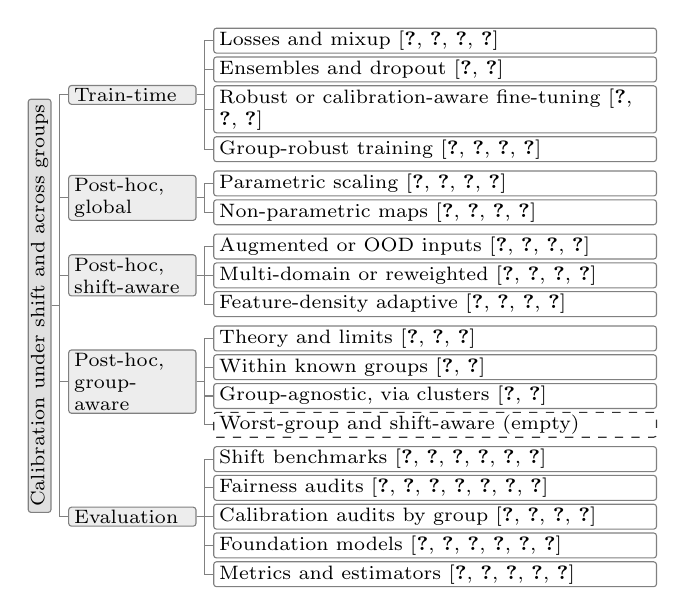
\begin{tikzpicture}[
      font=\scriptsize,
      line width=0.4pt,
      tax/.style={draw=black!50, rounded corners=1pt, align=left,
        inner xsep=2pt, inner ysep=1pt},
      branch/.style={tax, text width=42pt, fill=black!7},
      leaf/.style={tax, text width=156pt},
      fork/.style={draw=black!50}]
    %% Leaves, top to bottom: 1pt apart within a branch, 3pt between branches.
    \node[leaf] (t1) {Losses and mixup \cite{muller2019labelsmoothing,thulasidasan2019mixup,mukhoti2020focal,liu2022margin}};
    \node[leaf, below=1pt of t1] (t2) {Ensembles and dropout \cite{gal2016dropout,lakshminarayanan2017ensembles}};
    \node[leaf, below=1pt of t2] (t3) {Robust or calibration-aware fine-tuning \cite{kumar2022finetuning,oh2024calibrated,murugesan2024robust}};
    \node[leaf, below=1pt of t3] (t4) {Group-robust training \cite{sagawa2020groupdro,idrissi2022simple,shui2023clusterfocal,dutt2024fairtune}};
    \node[leaf, below=3pt of t4] (g1) {Parametric scaling \cite{platt1999probabilistic,guo2017calibration,kull2019dirichlet,tomani2022pts}};
    \node[leaf, below=1pt of g1] (g2) {Non-parametric maps \cite{zadrozny2002transforming,naeini2015bbq,zhang2020mixnmatch,gupta2021splines}};
    \node[leaf, below=3pt of g2] (s1) {Augmented or OOD inputs \cite{tomani2021posthoc,hekler2023tta,wang2024cascaded,roschewitz2025where}};
    \node[leaf, below=1pt of s1] (s2) {Multi-domain or reweighted \cite{wang2020transferable,gong2021confidence,yu2022multidomain,zou2023ace}};
    \node[leaf, below=1pt of s2] (s3) {Feature-density adaptive \cite{sun2022knn,tomani2023dac,yuksekgonul2023atypicality,kim2024energy}};
    \node[leaf, below=3pt of s3] (a1) {Theory and limits \cite{kleinberg2017inherent,pleiss2017fairness,liu2019implicit}};
    \node[leaf, below=1pt of a1] (a2) {Within known groups \cite{hebertjohnson2018multicalibration,shen2025calin}};
    \node[leaf, below=1pt of a2] (a3) {Group-agnostic, via clusters \cite{salvador2022faircal,yang2023beyond}};
    \node[leaf, below=1pt of a3, dashed, draw=black!80] (a4) {Worst-group and shift-aware (empty)};
    \node[leaf, below=3pt of a4] (e1) {Shift benchmarks \cite{hendrycks2019benchmarking,ovadia2019trust,minderer2021revisiting,wald2021calibration,disalvo2024medmnistc,roschewitz2025where}};
    \node[leaf, below=1pt of e1] (e2) {Fairness audits \cite{seyyedkalantari2021underdiagnosis,zhang2022improving,schrouff2022diagnosing,zong2023medfair,jin2024fairmedfm,ktena2024generative,yang2024limits}};
    \node[leaf, below=1pt of e2] (e3) {Calibration audits by group \cite{riccilara2023calibration,mehta2023evaluating,dominique2025calibration,xu2026demographic}};
    \node[leaf, below=1pt of e3] (e4) {Foundation models \cite{khan2023fair,tu2024empirical,hekler2025beyond,huang2026uncertainty,gupta2026subgroup,lin2026crsbench}};
    \node[leaf, below=1pt of e4] (e5) {Metrics and estimators \cite{brier1950verification,nixon2019measuring,kumar2019verified,roelofs2022mitigating,gruber2022proper}};
    %% Each branch sits 6pt left of its leaves, centered on its first and last leaf.
    \path ($(t1.west)!0.5!(t4.west)$) ++(-6pt,0) node[branch, anchor=east] (b1) {Train-time};
    \path ($(g1.west)!0.5!(g2.west)$) ++(-6pt,0) node[branch, anchor=east] (b2) {Post-hoc,\\global};
    \path ($(s1.west)!0.5!(s3.west)$) ++(-6pt,0) node[branch, anchor=east] (b3) {Post-hoc,\\shift-aware};
    \path ($(a1.west)!0.5!(a4.west)$) ++(-6pt,0) node[branch, anchor=east] (b4) {Post-hoc,\\group-aware};
    \path ($(e1.west)!0.5!(e5.west)$) ++(-6pt,0) node[branch, anchor=east] (b5) {Evaluation};
    %% The root reads bottom to top, so its south anchor faces the branches.
    \path ($(b1.west)!0.5!(b5.west)$) ++(-6pt,0) node[tax, fill=black!12, rotate=90, anchor=south] (root) {Calibration under shift and across groups};
    %% Forked edges that split 3pt to the right of the parent.
    \foreach \leaf in {t1,t2,t3,t4} \draw[fork] (b1.east) -- ++(3pt,0) |- (\leaf.west);
    \foreach \leaf in {g1,g2} \draw[fork] (b2.east) -- ++(3pt,0) |- (\leaf.west);
    \foreach \leaf in {s1,s2,s3} \draw[fork] (b3.east) -- ++(3pt,0) |- (\leaf.west);
    \foreach \leaf in {a1,a2,a3,a4} \draw[fork] (b4.east) -- ++(3pt,0) |- (\leaf.west);
    \foreach \leaf in {e1,e2,e3,e4,e5} \draw[fork] (b5.east) -- ++(3pt,0) |- (\leaf.west);
    \foreach \branch in {b1,b2,b3,b4,b5} \draw[fork] (root.south) -- ++(3pt,0) |- (\branch.west);
  \end{tikzpicture}
  \caption{Taxonomy of methods in the 82 surveyed papers. I found no published method for the dashed leaf, which is where GR-SATS belongs.}
  \Description{A tree that grows to the right. The root, calibration under shift and across groups, has five branches. Train-time methods, post-hoc global methods, post-hoc shift-aware methods, post-hoc group-aware methods, and evaluation work. Each branch ends in leaves that name a family of methods with its citations. One leaf under post-hoc group-aware, worst-group and shift-aware, has a dashed border because I found no published method for it.}
  \label{fig:taxonomy}
\end{figure}

Figure~\ref{fig:taxonomy} sorts the methods by when calibration happens and by what a post-hoc calibrator can depend on. Train-time methods change the loss, add mixup, or use ensembles and dropout, and they all need retraining. Of these, only Cluster-Focal \cite{shui2023clusterfocal} aims at group calibration, and group-robust training can even make uncertainty estimates worse \cite{mehta2023evaluating}. Global post-hoc methods such as temperature scaling (TS) \cite{guo2017calibration} fit one small mapping on clean validation data. Shift-aware post-hoc methods expose the calibrator to perturbed or out-of-distribution (OOD) data \cite{tomani2021posthoc,roschewitz2025where}, learn from several source domains \cite{gong2021confidence,yu2022multidomain}, or let the temperature depend on feature density, as DAC does with nearest-neighbor distances and AAR does with atypicality \cite{tomani2023dac,yuksekgonul2023atypicality}. Group-aware post-hoc methods calibrate within known groups \cite{hebertjohnson2018multicalibration,shen2025calin} or within clusters of embeddings when group labels are missing \cite{salvador2022faircal,yang2023beyond}. Over time these strands stayed mostly separate. Shift-aware calibrators appeared from 2020 on, while fairness work moved to worst-group training \cite{sagawa2020groupdro}, and since 2025 the work has become more critical, with Roschewitz et al.\ finding that calibrators built for shift do not reliably beat simpler ones \cite{roschewitz2025where}. None of the papers DAC cites deals with patient groups, and none of the papers FairMedFM cites is a calibration method. Table~\ref{tab:literature} compares ten representative works.

\begin{table*}[t]
  \caption{Comparison of representative related works. The two seed papers are in bold.}
  \label{tab:literature}
  \scriptsize
  \setlength{\tabcolsep}{3pt}
  \renewcommand{\arraystretch}{1.1}
  \begin{tabularx}{\textwidth}{@{}P{1.75cm}P{2.3cm}LP{1.9cm}P{1.85cm}LP{2.55cm}@{}}
    \toprule
    \textbf{Reference} & \textbf{Dataset} & \textbf{Method} & \textbf{Task} & \textbf{Metrics} & \textbf{Key finding} & \textbf{Limitation or gap} \\
    \midrule
    Ovadia 2019 \cite{ovadia2019trust} & MNIST, CIFAR-10-C, ImageNet-C, text, ad clicks, genomics & Benchmark of uncertainty methods such as TS, dropout, and ensembles & Classification under dataset shift & Accuracy, ECE, Brier, NLL & Calibration gets worse as shift grows, and ensembles hold up best & No groups and no medical images \\
    \addlinespace
    Tomani 2021 \cite{tomani2021posthoc} & CIFAR-10, ImageNet, ObjectNet & Post-hoc calibrators fit on a validation set perturbed with Gaussian noise & Image classification under domain drift & ECE, entropy & Standard calibrators are overconfident under drift, and the perturbation reduces this & One global mapping, assumes a noise-like shift \\
    \addlinespace
    \textbf{DAC} 2023 \cite{tomani2023dac} & CIFAR-10/100 and ImageNet with corruptions, ObjectNet-OOD & Per-image temperature from $k$-NN distances in several hidden layers & Image classification under shift and OOD & ECE, Brier, and others & Lowers ECE under corruption while keeping in-domain calibration & Average calibration only, no groups, no medical data \\
    \addlinespace
    AAR 2023 \cite{yuksekgonul2023atypicality} & ImageNet, CIFAR, MNLI, Fitzpatrick17k & Logit scale quadratic in atypicality, plus a bias for each class & Classification, including 9-class skin lesions & ECE, accuracy & Better worst skin-tone group without group labels & Fit for average NLL, clean data only \\
    \addlinespace
    FairCal 2022 \cite{salvador2022faircal} & RFW and BFW face pairs & One calibration map per k-means cluster of embeddings & Face verification & Accuracy, false positive rate gaps, group calibration & Fairer calibration without sensitive attributes or retraining & Faces only, no shift \\
    \addlinespace
    Cluster-Focal 2023 \cite{shui2023clusterfocal} & HAM10000, multiple sclerosis MRI & Cluster by calibration gap, then train with a group-wise focal loss & Skin lesions, multiple sclerosis activity & Worst-group quantile ECE, accuracy, F1 & Lower worst-subgroup calibration error with similar accuracy & Needs retraining, clean test data only \\
    \addlinespace
    \textbf{FairMedFM} 2024 \cite{jin2024fairmedfm} & 17 datasets, including HAM10000 and CheXpert & 20 foundation models with LP, parameter-efficient fine-tuning, and CLIP-based adaptation & Classification and segmentation & AUC, AUC gap, equalized odds, ECE gap, Dice & Bias is common, and mitigation helps little & Clean in-distribution tests only, no calibration method \\
    \addlinespace
    MedMNIST-C 2024 \cite{disalvo2024medmnistc} & 12 MedMNIST+ datasets & Modality-specific corruptions at five severities & Classification robustness & Balanced error, AUC & Corruptions cut performance, and corruption augmentation helps & No calibration metrics, no groups \\
    \addlinespace
    Roschewitz 2025 \cite{roschewitz2025where} & 8 tasks with natural shift, 4 of them medical & Comparison of post-hoc and in-training calibration & Image classification under natural shift & ECE, Brier & OOD exposure is most robust, and shift-specific methods do not reliably beat simple ones & No subgroups, no graded corruption \\
    \addlinespace
    Dominique 2025 \cite{dominique2025calibration} & ISIC 2020, PROVE-AI & Audit of the top three ISIC 2020 models & Melanoma detection & AUC, calibration by group & Models overestimate risk and are miscalibrated across sex, skin tone, and age & Audit only, no fix \\
    \bottomrule
  \end{tabularx}
\end{table*}

\subsection{Limitations of Existing Work}

Table~\ref{tab:literature} shows the pattern behind this project. The papers that handle shift \cite{ovadia2019trust,tomani2021posthoc,tomani2023dac,roschewitz2025where,hekler2023tta} measure or improve only average calibration and report nothing by patient group. The papers that handle groups need retraining \cite{shui2023clusterfocal}, were built for a different task without shift \cite{salvador2022faircal}, or only audit existing models \cite{dominique2025calibration}. AAR comes closest, since it helped the worst skin-tone group without group labels, but it optimizes average NLL and was only tested on clean images \cite{yuksekgonul2023atypicality}. Studies of calibration in adapted or foundation models focus on CLIP and natural images \cite{tu2024empirical,oh2024calibrated,murugesan2024robust} or do not report groups \cite{hekler2025beyond,huang2026uncertainty,lin2026crsbench}, and Gupta et al.\ compared adapters by subgroup performance but not calibration \cite{gupta2026subgroup}. Finally, group calibration is usually summarized with a gap in binned expected calibration error (ECE), which is unreliable for small groups \cite{kumar2019verified,riccilara2023calibration}.

%% =========================================================
\section{Research Challenges and Motivation}
\label{sec:challenges}

These limitations point to three challenges. Each one is tied to a component of the method in Section~\ref{sec:method}, as summarized in Table~\ref{tab:mapping}.

\subsection{Challenge 1: Protecting the Worst-Off Group Under Shift}
\label{sec:ch1}

\textbf{Problem:} I need a calibrator that keeps every patient group, and the worst-off one in particular, calibrated when test images are corrupted, without knowing anyone's group at test time. I target calibration within each group and not equal error rates, since the two generally cannot hold together \cite{pleiss2017fairness}.

\textbf{Evidence from literature:} Every shift-aware calibrator in Figure~\ref{fig:taxonomy} is fit for average calibration \cite{tomani2021posthoc,yu2022multidomain,tomani2023dac,kim2024energy}, and every group-aware post-hoc calibrator assumes that calibration and test data come from the same distribution \cite{hebertjohnson2018multicalibration,salvador2022faircal,shen2025calin}. Cluster-Focal lowers the worst subgroup's calibration error, but it is a training loss and needs a new model \cite{shui2023clusterfocal}.

\textbf{Importance:} A calibrator tuned for the average can get most of its gains from the large groups while the smallest group stays overconfident. In dermatology the smallest groups are often patients with darker skin \cite{groh2021fitzpatrick}.

\textbf{Technical difficulty:} Without group labels at test time, a calibrator can only treat a group differently if that group's images look different in what the calibrator sees, here the logit and the feature distance. The worst-group objective is a maximum of group losses, so it is not smooth, and a flexible calibrator can overfit a group with only 10 validation cancers. DAC puts its linear model on the temperature, which makes a worst-group DAC non-convex. Lowering the worst group's loss can also raise the other groups' losses, the leveling down that MEDFAIR warns about \cite{zong2023medfair}.

\textbf{Connection to proposed method:} The worst-group fit (C3) of an inverse temperature that is linear in the shift score (C2) stays convex with only two parameters, and per-group reporting makes any leveling down visible.

\subsection{Challenge 2: A Shift Signal That Transfers}
\label{sec:ch2}

\textbf{Problem:} The calibrator has to tell how far a test image is from the training data in a way that keeps working on corruptions it never saw and on models adapted in different ways.

\textbf{Evidence from literature:} Tomani et al.'s fix assumes that the shift looks like Gaussian noise \cite{tomani2021posthoc}, DAC uses raw distances from many layers \cite{tomani2023dac}, and calibrators built for shift do not reliably beat simple ones under natural shift \cite{roschewitz2025where}. MedMNIST-C and CRS-Bench measure corruption robustness without looking at groups \cite{disalvo2024medmnistc,lin2026crsbench}, and FairMedFM compares adaptation strategies only on clean data \cite{jin2024fairmedfm}, even though fine-tuning can distort pretrained features \cite{kumar2022finetuning}.

\textbf{Importance:} Nobody knows in advance which corruptions a deployed model will see, so a calibrator that only works on the corruptions it was fit on gives a false sense of safety.

\textbf{Technical difficulty:} Raw distances have different scales for different backbones and adaptation strategies, and fine-tuning pulls training features closer together, so distances among training images understate how far a new clean image is. A percentile of clean distances tops out once corruption pushes an image past every clean image. A temperature that is linear in the score can extrapolate to a negative or huge value on a new corruption. The score is also confounded with group, because groups that are rare in training sit farther from the training data even on clean images.

\textbf{Connection to proposed method:} The standardized and clipped log-distance score (C1) handles scale and saturation, leave-one-family-out testing (Section~\ref{sec:splits}) checks transfer, and a group-balanced reference bank separates the confound (Section~\ref{sec:failure}).

\subsection{Challenge 3: Fitting and Evaluating Small Groups}
\label{sec:ch3}

\textbf{Problem:} The groups that matter most have very few positive cases, so both fitting a worst-group calibrator and judging whether it helps are noisy.

\textbf{Evidence from literature:} In the Fitzpatrick17k-C splits \cite{abhishek2025quality}, skin types V and VI have 10 validation cancers and 22 test cancers. Binned ECE is biased when samples are few \cite{kumar2019verified,roelofs2022mitigating}, which can lead to wrong fairness conclusions \cite{riccilara2023calibration}, yet FairMedFM summarizes calibration fairness with a single ECE gap \cite{jin2024fairmedfm}.

\textbf{Importance:} Without a careful protocol, a method could look better or worse for the darkest skin types purely by chance.

\textbf{Technical difficulty:} The bias of binned ECE depends on the number of samples and bins, so ECE values for groups of 362 and 1,794 images are not comparable. Fitting on the validation split alone leaves 10 cancers for the worst group. About 75 corrupted copies share one source image, so treating them as independent makes confidence intervals far too narrow, and testing every pair of more than ten methods over 8 settings invites false positives.

\textbf{Connection to proposed method:} Cross-fitting over the pooled validation and test images (Section~\ref{sec:splits}) gives every fit and every test more cases. NLL and Brier score are the primary metrics, and three pre-specified comparisons are tested with a paired bootstrap over source images (Section~\ref{sec:metrics}).

%% =========================================================
\section{Proposed Methodology}
\label{sec:method}

\begin{figure*}[t]
  \centering
  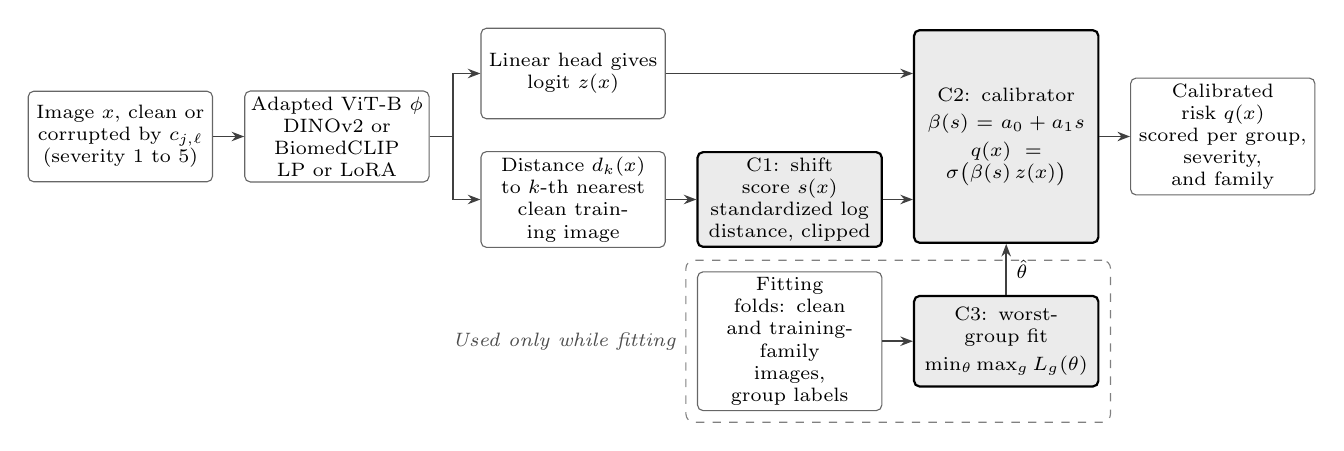
\begin{tikzpicture}[
      font=\scriptsize,
      blk/.style={draw=black!60, rounded corners=2pt, align=center,
        text width=2.2cm, minimum height=1.15cm, inner sep=2pt},
      mine/.style={blk, fill=black!8, draw=black, thick},
      arr/.style={-{Stealth[length=1.6mm]}, semithick, draw=black!75}]
    \node[blk] (input) at (0,0) {Image $x$, clean or\\corrupted by $c_{j,\ell}$\\(severity 1 to 5)};
    \node[blk] (enc) at (2.75,0) {Adapted ViT-B $\phi$\\DINOv2 or BiomedCLIP\\LP or LoRA};
    \node[blk] (logit) at (5.75,0.8) {Linear head gives\\logit $z(x)$};
    \node[blk] (knn) at (5.75,-0.8) {Distance $d_k(x)$\\to $k$-th nearest\\clean training image};
    \node[mine] (score) at (8.5,-0.8) {C1: shift score $s(x)$\\standardized log\\distance, clipped};
    \node[mine, minimum height=2.7cm] (cal) at (11.25,0) {C2: calibrator\\[2pt]$\beta(s) = a_0 + a_1 s$\\[2pt]$q(x) = \sigma\big(\beta(s)\, z(x)\big)$};
    \node[blk] (risk) at (14.0,0) {Calibrated risk $q(x)$\\scored per group,\\severity, and family};
    \node[blk] (fitdata) at (8.5,-2.6) {Fitting folds: clean\\and training-family\\images, group labels};
    \node[mine] (obj) at (11.25,-2.6) {C3: worst-group fit\\[2pt]$\min_{\theta}\max_{g} L_g(\theta)$};
    \node[draw=black!50, dashed, rounded corners=3pt, inner sep=4pt, fit=(fitdata)(obj),
      label={[font=\scriptsize\itshape, text=black!70]left:Used only while fitting}] {};
    \draw[arr] (input) -- (enc);
    \draw[arr] (enc.east) -- ++(0.3,0) |- (logit.west);
    \draw[arr] (enc.east) -- ++(0.3,0) |- (knn.west);
    \draw[arr] (logit.east) -- (logit.east -| cal.west);
    \draw[arr] (knn) -- (score);
    \draw[arr] (score.east) -- (score.east -| cal.west);
    \draw[arr] (cal) -- (risk);
    \draw[arr] (fitdata) -- (obj);
    \draw[arr] (obj) -- node[right] {$\hat{\theta}$} (cal);
  \end{tikzpicture}
  \caption{Overview of the proposed methodology. Shaded blocks are the proposed components of Section~\ref{sec:components}. Group labels are used only in the dashed fitting step, so at test time the calibrator needs only the image and the adapted model.}
  \Description{A flow diagram. An image, clean or corrupted, goes into an adapted ViT-B backbone. The backbone feeds a linear head that gives a logit, and a nearest-neighbor distance to clean training images. The distance becomes a standardized shift score. The logit and the shift score go into the calibrator, which computes an inverse temperature from the score and rescales the logit to give a calibrated risk that is scored per group and severity. Below, inside a dashed box labeled used only while fitting, fitting folds with group labels feed a worst-group fit that sends the fitted parameters up to the calibrator.}
  \label{fig:framework}
\end{figure*}

GR-SATS is a post-hoc calibrator. It takes an adapted model's logit and feature vector for one image and outputs a calibrated probability that the lesion is malignant. A shift score (C1) measures how far the features are from clean training features, a calibrator (C2) turns that score into an inverse temperature that rescales the logit, and a worst-group fit (C3) picks the calibrator's two parameters. A fourth component (C4), DAC fit for the worst group, separates the effect of the objective from the effect of the parameterization.

\subsection{Problem Formulation}
\label{sec:formulation}

Each example is an image $x$ with a label $y \in \{0,1\}$, where $y = 1$ means malignant. Let $\mathcal{G}$ be a set of patient groups. For Fitzpatrick17k it holds the skin-type groups I-II, III-IV, and V-VI, and for HAM10000 it holds four overlapping groups (female, male, under 60, and 60 or older). An adapted model $f = h \circ \phi$ has a backbone $\phi$ that maps an image to a feature vector $v(x)$ and a linear head $h$ that gives a logit $z(x)$. A corruption $c_{j,\ell}$ applies corruption type $j$ at severity $\ell \in \{1, \dots, 5\}$, with $\ell = 0$ meaning clean, and each type belongs to one of five families. A post-hoc calibrator $q_\theta$ maps $z(x)$ and $v(x)$ to a calibrated probability $q_\theta(x)$ without seeing $y$ or the group. It is fit on labeled clean and corrupted images from some corruption families and tested on a family that was left out. The goal is calibration within every group under this shift,
\begin{equation}
  \Pr\big(Y = 1 \mid q_\theta(X) = p,\ X \in g\big) \approx p,
  \label{eq:goal}
\end{equation}
for every $p \in [0,1]$ and every $g \in \mathcal{G}$. Equation~\eqref{eq:goal} cannot be checked directly with small groups, so I measure it with each group's NLL and Brier score and focus on the worst group.

\subsection{Overall Framework}

Figure~\ref{fig:framework} shows the pipeline. An image, clean or corrupted with a MedMNIST-C corruption, goes through the adapted backbone. The head gives the logit $z$, and the feature $v$ is compared with a bank of clean training features to get the shift score (C1). The calibrator rescales the logit with a score-dependent inverse temperature (C2) whose two parameters come from the worst-group fit (C3), which is the only step that uses group labels.

\subsection{Proposed Components}
\label{sec:components}

\textbf{C1. Standardized shift score.} Following DAC \cite{tomani2023dac}, the score starts from the Euclidean distance $d_k(x)$ between the L2-normalized feature $v(x)$ and its $k$-th nearest neighbor in a bank of normalized clean training features. Unlike DAC, I use one layer, the feature the head receives, and standardize the log distance,
\begin{equation}
  s(x) = \operatorname{clip}\left(\frac{\log d_k(x) - m}{r},\ s_{\min},\ s_{\max}\right),
  \label{eq:score}
\end{equation}
where $m$ and $r$ are the mean and standard deviation of $\log d_k$ over the clean fitting images and $[s_{\min}, s_{\max}]$ is the range of scores seen during fitting. The log makes the skewed distances more symmetric, and standardizing with clean fitting images makes the score unitless, so one calibrator design works for both backbones and both adaptation strategies, and it avoids the way fine-tuning pulls training features together. The clipping keeps a new corruption from pushing the temperature outside the fitted range. Because the bank comes from the training split, a corrupted image is never matched with its own clean copy. This component addresses Challenge 2.

\textbf{C2. Shift-dependent inverse temperature.} The calibrated probability is
\begin{equation}
  q_\theta(x) = \sigma\big(\beta_\theta(s(x))\, z(x)\big), \qquad \beta_\theta(s) = a_0 + a_1 s,
  \label{eq:calib}
\end{equation}
where $\sigma$ is the sigmoid and $\theta = (a_0, a_1)$ is in the set $\Theta$ where $\beta_\theta(s_{\min}) \geq \epsilon$ and $\beta_\theta(s_{\max}) \geq \epsilon$. Since $\beta_\theta$ is linear, these two constraints keep it positive on the whole clipped range, so the predicted class at the 0.5 threshold never changes, and $a_1 = 0$ gives ordinary TS. DAC instead makes the temperature itself linear in distances. Putting the linear model on the inverse temperature is what makes the worst-group fit convex, which is how this component serves Challenge 1. A temperature cannot fix risks that are too high or too low across the board, which the base-rate gaps in Section~\ref{sec:data} make likely, so I also test a bias variant, $\sigma(\beta_\theta(s)\, z + b_0 + b_1 s)$. Its fit is still convex, but it can change predictions, so I report the area under the ROC curve (AUC) and accuracy for it and pick the main version at the go/no-go point (Section~\ref{sec:gonogo}).

\textbf{C3. Worst-group objective.} Let $D_{g,\ell}$ be the fitting images of group $g$ at severity $\ell$, where severities 1 to 5 use only the training corruption families. The loss of group $g$ and the fit are
\begin{equation}
  L_g(\theta) = \frac{1}{6}\sum_{\ell=0}^{5}\frac{1}{|D_{g,\ell}|}\sum_{(x,y)\in D_{g,\ell}} -\log q_\theta(y \mid x),
  \label{eq:grouploss}
\end{equation}
\begin{equation}
  \hat{\theta} = \arg\min_{\theta \in \Theta}\ \max_{g \in \mathcal{G}}\ L_g(\theta),
  \label{eq:objective}
\end{equation}
with $q_\theta(1 \mid x) = q_\theta(x)$ and $q_\theta(0 \mid x) = 1 - q_\theta(x)$, as in GroupDRO \cite{sagawa2020groupdro}. Each $L_g$ averages logistic losses of $\beta_\theta(s)\, z$, which is linear in $\theta$, so each $L_g$ and their maximum are convex and $\Theta$ is set by linear constraints. I therefore solve Eq.~\eqref{eq:objective} exactly in epigraph form, minimizing $t$ subject to $L_g(\theta) \leq t$ for every group. The factor $1/6$ gives clean images and each severity the same weight, so the 55 to 65 corrupted copies of each image do not swamp the clean one. Raw NLL also reflects how hard a group is to classify, so a second version minimizes the excess loss $L_g(\theta) - \min_{\theta' \in \Theta} L_g(\theta')$. This component addresses Challenge 1, and it is what separates GR-SATS from DAC and AAR, which are both fit for average calibration.

\textbf{C4. DAC fit for the worst group.} The approved idea was to change DAC so that it targets the worst group, so I also test this literal version, which I call DAC-WG. It keeps DAC's temperature $S_w(x) = w_0 + \sum_l w_l\, d_k^{(l)}(x)$, a weighted sum of $k$-NN distances with positive weights over the layers DAC uses for ViT-Base. DAC fits $w$ by minimizing the average squared error (the Brier score) on the validation set, and DAC-WG fits it with Eq.~\eqref{eq:objective} instead. This loss is not convex in $w$, so I use GroupDRO's alternating gradient and exponentiated-gradient updates \cite{sagawa2020groupdro}. Comparing DAC with DAC-WG shows the effect of the objective, and comparing DAC-WG with GR-SATS isolates the parameterization.

\textbf{Why this design.} The worst group in Fitzpatrick17k has a few dozen cancers even after pooling, so a calibrator with many parameters would likely overfit it. Retraining methods such as GroupDRO or Cluster-Focal would need a new model for every attribute and adaptation strategy, while a post-hoc calibrator runs on saved outputs in seconds. Group-wise TS needs group labels at test time, which are often missing or sensitive, so I only use it as a reference.

\begin{table}[t]
  \caption{Mapping between research challenges and proposed methods.}
  \label{tab:mapping}
  \scriptsize
  \setlength{\tabcolsep}{3pt}
  \renewcommand{\arraystretch}{1.1}
  \begin{tabularx}{\columnwidth}{@{}P{1.3cm}LLL@{}}
    \toprule
    \textbf{Challenge} & \textbf{Technique} & \textbf{Function} & \textbf{Expected effect} \\
    \midrule
    1. Worst-off group under shift & Worst-group fit (C3) of an inverse temperature linear in the shift score (C2) & Picks the two parameters that minimize the largest group loss, as a convex problem & Lower worst-group NLL and Brier score under corruption \\
    \addlinespace
    2. Shift signal that transfers & Standardized, clipped log $k$-NN distance (C1), leave-one-family-out testing & Gives a unitless score that grows with severity and stays in the fitted range & Calibration that holds on unseen corruption families, for LP and LoRA \\
    \addlinespace
    3. Small groups & Cross-fitting, proper scores, paired bootstrap over source images & Uses every pooled image for testing and gives honest uncertainty & Conclusions about small groups that are not driven by noise \\
    \bottomrule
  \end{tabularx}
\end{table}

%% =========================================================
\section{Experimental Methodology}
\label{sec:experiments}

\subsection{Dataset}
\label{sec:data}

I use two public image datasets with binary malignancy labels and patient group labels. HAM10000 \cite{tschandl2018ham10000} has 10,015 dermoscopic images of 7,470 lesions with the patient's sex and age.\footnote{\url{https://doi.org/10.7910/DVN/DBW86T}} I use the splits of DermaMNIST-C \cite{abhishek2025quality}, a corrected version of DermaMNIST in which no lesion crosses splits (the C stands for corrected, not corrupted). Melanoma, basal cell carcinoma, and actinic keratosis or intraepithelial carcinoma are malignant, and everything else is benign. MEDFAIR counts basal cell carcinoma as benign \cite{zong2023medfair}, but it is a skin cancer, so I keep the clinical definition. The groups are sex and age, split at 60 as in MEDFAIR. Fitzpatrick17k \cite{groh2021fitzpatrick} has 16,577 clinical photos of 114 skin conditions with Fitzpatrick skin types. I use the cleaned Fitzpatrick17k-C \cite{abhishek2025quality}, which has 11,394 images with fixed splits.\footnote{\url{https://doi.org/10.5281/zenodo.11101337}} The label is malignant versus everything else, as in MEDFAIR, and I merge the six skin types into I-II, III-IV, and V-VI so that each group has enough cases.

Following MEDFAIR, I drop images whose group attribute was not recorded (67 in HAM10000 and 296 in Fitzpatrick17k-C), which leaves no missing values and gives HAM10000 the same 9,948 images that MEDFAIR and FairMedFM use \cite{zong2023medfair,jin2024fairmedfm}. Table~\ref{tab:data} gives the counts. Two features of the data matter for calibration. In HAM10000, lesions with several photos ended up almost entirely in the training split (1,876 of 1,956) and are more often malignant, so 21.3\% of training images are malignant compared with 11.9\% of the pooled validation and test images. In Fitzpatrick17k-C, 8.8\% of the pooled V-VI images are malignant compared with 16.0\% of the I-II images.

For shift I use the 15 dermatology corruptions of MedMNIST-C \cite{disalvo2024medmnistc} at five severities.\footnote{\url{https://github.com/francescodisalvo05/medmnistc-api}} They fall into five families, digital (JPEG and pixelate), noise (Gaussian, speckle, impulse, and shot), blur (defocus, motion, and zoom), color (brightness and contrast, each up and down), and task-specific (black corners and text overlays). The task-specific family imitates dermoscope artifacts, so for Fitzpatrick17k's clinical photos I report it separately.

\begin{table}[t]
  \caption{Data after removing images with an unrecorded group attribute. Each entry is the number of images, with malignant cases in parentheses. The pool is the validation and test splits together, used through 5-fold cross-fitting.}
  \label{tab:data}
  \footnotesize
  \begin{tabular}{@{}lrr@{}}
    \toprule
     & \textbf{HAM10000} & \textbf{Fitzpatrick17k-C} \\
    \midrule
    Training split & 8,164 (1,740) & 7,779 (1,144) \\
    Validation split & 568 (63) & 1,100 (154) \\
    Test split & 1,216 (149) & 2,219 (325) \\
    Pool & 1,784 (212) & 3,319 (479) \\
    \midrule
    \multicolumn{3}{@{}l}{\textit{Groups in the pool}} \\
    Female & 820 (80) & \\
    Male & 964 (132) & \\
    Age under 60 & 1,206 (62) & \\
    Age 60 or older & 578 (150) & \\
    Skin type I-II & & 1,794 (287) \\
    Skin type III-IV & & 1,163 (160) \\
    Skin type V-VI & & 362 (32) \\
    \bottomrule
  \end{tabular}
\end{table}

\subsection{Data Preprocessing}

Every image is resized to a shorter side of 224 pixels and center-cropped to 224 by 224, the resolution MedMNIST-C's corruption settings were designed for \cite{disalvo2024medmnistc}. Corruptions are applied to this crop, and the result is normalized with each backbone's mean and standard deviation. Each corrupted image is generated from a seed made of the image, the corruption, and the severity, so every model sees exactly the same corrupted images and they can be rebuilt instead of stored. Training uses only geometric augmentation (random resized crops with scale 0.8 to 1, flips, and 90-degree rotations), since color and blur augmentation would overlap with the test corruptions. I do not reweight the classes, since that would push predicted probabilities away from the true rates. Everything learned from data, including the probes, the reference bank, the score standardization, and every calibrator, uses only the training split or the fitting folds.

\subsection{Data Splitting and Validation}
\label{sec:splits}

Models are trained on the official training split, with 10\% held out (grouped by lesion for HAM10000) as a development slice for early stopping and choosing the probe's regularization. The validation and test splits are pooled and split into five folds, stratified by group and label, with all images of a lesion and all corrupted copies of an image kept in the same fold. For each fold $f$ and each corruption family $h$, a calibrator is fit on the clean images outside $f$ and their copies corrupted by the other four families, and then tested on the clean images in $f$ and their copies corrupted by $h$. So every pooled image is tested once for each family by a calibrator that never saw that image or that family. Each fit sees more than twice as many images as the validation split alone, and the final metrics use the whole pool, which for skin types V and VI is 362 images and 32 cancers. Every model is trained with three seeds, which also change the development slice.

\subsection{Baseline Methods}
\label{sec:baselines}

\begin{itemize}
  \item \textbf{Baseline 1, simple global calibrators.} No calibration, TS fit on clean images \cite{guo2017calibration}, TS fit on images perturbed with Gaussian noise \cite{tomani2021posthoc}, TS fit on clean images plus my training corruption families, and TS with exposure to unrelated texture images, which Roschewitz et al.\ found most robust under natural shift \cite{roschewitz2025where}.
  \item \textbf{Baseline 2, shift-aware calibrators.} DAC \cite{tomani2023dac}, multi-domain TS \cite{yu2022multidomain}, and AAR \cite{yuksekgonul2023atypicality}, all fit on the same clean and corrupted images as my method.
  \item \textbf{Baseline 3, group-aware calibrators.} Cluster-wise TS in the style of FairCal \cite{salvador2022faircal}, which fits one temperature per k-means cluster and needs no test-time group labels. Group-wise TS and a per-group version of GR-SATS use test-time group labels, so they serve only as oracles.
\end{itemize}

TS with my corruption families is the strongest simple baseline. DAC is the seed method and AAR is the closest existing method, so these three are the primary comparisons.

\subsection{Implementation Details}

I will write the code in Python with PyTorch. The backbones are DINOv2 ViT-B/14 \cite{oquab2024dinov2}, which is self-supervised on 142 million natural images, and the ViT-B/16 image encoder of BiomedCLIP \cite{zhang2025biomedclip}, a CLIP-style model \cite{radford2021clip} trained on 15 million biomedical figure and caption pairs. Both are ViT-Base models \cite{dosovitskiy2021vit} in FairMedFM, so pretraining is the main difference between them. LP is an L2-regularized logistic regression on the frozen embedding, with the strength chosen from $\{0.01, 0.1, 1, 10\}$ by development-slice NLL. LoRA \cite{hu2022lora} adds rank-8 adapters with scaling 16 to the query and value projections, plus a linear head, trained with unweighted binary cross-entropy and AdamW (learning rate $3 \times 10^{-4}$, weight decay 0.01, batch size 64, cosine schedule) for at most 20 epochs, keeping the epoch with the lowest development-slice NLL. Nearest neighbors come from FAISS with $k = 10$, GR-SATS is solved with CVXPY with $\epsilon = 0.05$, cluster-wise TS uses 8 clusters, and DAC and AAR use their official code.\footnote{\url{https://github.com/futakw/DensityAwareCalibration} and \url{https://github.com/mertyg/beyond-confidence-atypicality}} Training runs on free Google Colab T4 GPUs with mixed precision, with Kaggle as a backup. Jobs checkpoint to Google Drive so they survive disconnects, and each corrupted batch is generated once and passed through every model of the same dataset, since the two CPU cores are the bottleneck. The calibrators only need saved logits and distances, so they fit on a CPU in seconds to minutes. I estimate the core grid at 10 to 20 T4 hours.

\subsection{Evaluation Metrics}
\label{sec:metrics}

\textbf{Primary metrics.} The main test pools the held-out corruption families at severities 3 to 5, where calibration is most likely to fail, and leaves out the task-specific family for Fitzpatrick17k. On this pool I report worst-group NLL and worst-group Brier score, taking the worst group over all four HAM10000 groups and also per attribute. Both are proper scoring rules \cite{brier1950verification,gruber2022proper}, so a method cannot improve them without better probabilities. Unlike binned ECE, they need no bins and are not biased upward in small groups \cite{kumar2019verified,roelofs2022mitigating}.

\textbf{Secondary metrics.} Per-group NLL and Brier score show whether a method narrows the gap by making the better-off groups worse \cite{zong2023medfair}, and average NLL shows what the worst-group fit costs. ECE uses 15 equal-mass bins \cite{roelofs2022mitigating} alongside the debiased estimator of Kumar et al.\ \cite{kumar2019verified}. I also report the ECE gap between groups, AUC, since a per-image temperature can reorder images, and accuracy for methods that can change predictions. On clean images, ECE and AUC measure the in-distribution cost that Roschewitz et al.\ warn about \cite{roschewitz2025where}.

\textbf{Statistics.} GR-SATS succeeds against a primary comparison if it has lower worst-group NLL and Brier score averaged over the 8 settings, with a 95\% paired bootstrap interval that excludes zero. The bootstrap resamples source images 2,000 times (lesions for HAM10000), since the corrupted copies of one image are not independent. I also expect GR-SATS to close at least half of the worst-group NLL gap to the per-group oracle and to stay within 0.01 ECE and 1 AUC point of clean TS on clean images. To rank all methods across settings without dozens of pairwise tests, I use the Friedman test with the Nemenyi post-hoc test, as MEDFAIR does \cite{zong2023medfair}.

%% =========================================================
\section{Results and Analysis}
\label{sec:results}

No experiments have been run yet, so every entry below is to be determined (TBD).

\subsection{Main Results}

\begin{table}[t]
  \caption{Planned main results on unseen corruption families at severities 3 to 5, averaged over the 8 settings. WG means worst group, and $\dagger$ marks oracles that use group labels at test time.}
  \label{tab:results}
  \scriptsize
  \setlength{\tabcolsep}{3.5pt}
  \begin{tabular}{@{}lccccc@{}}
    \toprule
    \textbf{Method} & \textbf{WG NLL} & \textbf{WG Brier} & \textbf{NLL} & \textbf{Clean ECE} & \textbf{AUC} \\
    \midrule
    No calibration & TBD & TBD & TBD & TBD & TBD \\
    TS, clean & TBD & TBD & TBD & TBD & TBD \\
    TS with Gaussian noise & TBD & TBD & TBD & TBD & TBD \\
    TS with corruptions & TBD & TBD & TBD & TBD & TBD \\
    TS with textures & TBD & TBD & TBD & TBD & TBD \\
    DAC & TBD & TBD & TBD & TBD & TBD \\
    Multi-domain TS & TBD & TBD & TBD & TBD & TBD \\
    AAR & TBD & TBD & TBD & TBD & TBD \\
    Cluster-wise TS & TBD & TBD & TBD & TBD & TBD \\
    GR-SATS (proposed) & TBD & TBD & TBD & TBD & TBD \\
    \midrule
    Group-wise TS$^\dagger$ & TBD & TBD & TBD & TBD & TBD \\
    Per-group GR-SATS$^\dagger$ & TBD & TBD & TBD & TBD & TBD \\
    \bottomrule
  \end{tabular}
\end{table}

Table~\ref{tab:results} will hold the main comparison. I will test three hypotheses. \textbf{H1.} The worst-group NLL of clean-fit TS rises with severity, and faster for the worst group than for the best one. \textbf{H2.} The severity at which clean-fit TS starts doing harm, meaning a higher worst-group NLL than no calibration, differs between LP and LoRA. \textbf{H3.} GR-SATS meets the success criteria of Section~\ref{sec:metrics} against all three primary comparisons. H1 and H2 are measurements, so they are worth reporting whatever happens with H3.

\subsection{Ablation Study}

\begin{table}[t]
  \caption{Planned ablation on the same test pool. The first four rows cross a global or shift-aware temperature with an average or worst-group loss.}
  \label{tab:ablation}
  \scriptsize
  \begin{tabular}{@{}llcc@{}}
    \toprule
    \textbf{Temperature} & \textbf{Loss} & \textbf{WG NLL} & \textbf{NLL} \\
    \midrule
    Global & Average (TS with corruptions) & TBD & TBD \\
    Global & Worst group & TBD & TBD \\
    Shift-aware & Average & TBD & TBD \\
    Shift-aware & Worst group (GR-SATS) & TBD & TBD \\
    \midrule
    \multicolumn{2}{@{}l}{GR-SATS with excess NLL} & TBD & TBD \\
    \multicolumn{2}{@{}l}{GR-SATS with bias term} & TBD & TBD \\
    \multicolumn{2}{@{}l}{DAC, average squared error} & TBD & TBD \\
    \multicolumn{2}{@{}l}{DAC-WG, worst-group NLL} & TBD & TBD \\
    \bottomrule
  \end{tabular}
\end{table}

If the shift-aware, worst-group cell of Table~\ref{tab:ablation} beats both cells that change only one part, then both parts matter. If the worst-group loss also helps DAC, the gain comes from the objective and not from my shift score. I will also check sensitivity to $k \in \{1, 10, 50\}$.

\subsection{Error and Failure Analysis}
\label{sec:failure}

Per-group reliability diagrams at each severity will show whether errors come from overconfidence, which a temperature can fix, or from risks that are off in one direction, which needs the bias variant. Per-family results will show which corruptions break the calibrator, for example whether brightness and contrast changes hurt darker skin types more. To tell whether a group has high shift scores because of corruption or just because it is rare in training, I will check whether the gap in scores between groups grows beyond its clean value and rerun the method with a reference bank that has equal numbers from each group.

%% =========================================================
\section{Project Execution Plan}
\label{sec:plan}

\subsection{Six-Week Research and Implementation Plan}

Table~\ref{tab:plan} lists the weekly objectives, tasks, and milestones from October 19 to November 29, 2026.

\begin{table*}[t]
  \caption{Six-week research and implementation plan.}
  \label{tab:plan}
  \scriptsize
  \setlength{\tabcolsep}{4pt}
  \renewcommand{\arraystretch}{1.15}
  \begin{tabularx}{\textwidth}{@{}P{1.3cm}P{2.1cm}LP{4.6cm}P{1.15cm}@{}}
    \toprule
    \textbf{Week} & \textbf{Objective} & \textbf{Specific tasks} & \textbf{Expected output or milestone} & \textbf{Member} \\
    \midrule
    1 (Oct 19 to 25) & Data pipeline and linear probes & Write loaders with the label and group rules of Section~\ref{sec:data}, set up Colab notebooks that resume after a disconnect, build the folds, set up the 15 corruptions with per-image seeds, and train linear probes on frozen features with three seeds. & Counts that match Table~\ref{tab:data}, no lesion in two folds, and clean AUC for all 12 linear probes. & Adit Patel \\
    \addlinespace
    2 (Oct 26 to Nov 1) & LoRA models and pilot & Train the 12 LoRA models, save logits and distances for all clean and corrupted pooled images, fit clean TS, plot per-group NLL and ECE against severity, and run the pilot check of Section~\ref{sec:gonogo} with a quick worst-group fit. & Pilot report and a written go/no-go decision with the choice of main variant by November 1. & Adit Patel \\
    \addlinespace
    3 (Nov 2 to 8) & Method and baselines & Implement GR-SATS, its variants, DAC-WG, and the baselines, plus the cross-fitting harness with unit tests (zero slope gives TS, no flipped predictions, disjoint folds). & Every calibrator runs on one setting, and my TS and DAC numbers match the official code there. & Adit Patel \\
    \addlinespace
    4 (Nov 9 to 15) & Main experiments & Run every calibrator on the 8 settings with three seeds, and compute all metrics, bootstrap intervals, and the Friedman and Nemenyi tests. & Filled Table~\ref{tab:results} and a verdict on H1 to H3. & Adit Patel \\
    \addlinespace
    5 (Nov 16 to 22) & Ablation and failure analysis & Fill Table~\ref{tab:ablation} with the $k$ sensitivity check, and run the analyses of Section~\ref{sec:failure}. & Ablation table, reliability diagrams, and a written analysis of why the method helps or fails. & Adit Patel \\
    \addlinespace
    6 (Nov 23 to 29) & Final paper and reproducibility & Rerun one setting from scratch, write the results, discussion, and limitations, and prepare the poster. & Final paper, poster, and runnable code with setup and data instructions that rebuild every table. & Adit Patel \\
    \bottomrule
  \end{tabularx}
\end{table*}

\subsection{Go/No-Go Decision and Scope}
\label{sec:gonogo}

Ordinary training often gives group calibration on its own \cite{liu2019implicit}, so at the end of Week 2 I first check that there is something to fix. The pilot passes if, on at least one dataset, the worst-group fit lowers worst-group NLL by more than one bootstrap standard error compared with the average fit when both are fit directly on the evaluation images, and the worst group's mean shift score differs from the other groups' at severities 3 to 5. If neither dataset passes, I will switch to the measurement study, which reports the severity at which clean-fit calibration starts doing harm under each adaptation strategy. If the core grid finishes early, I will add an ImageNet-supervised ViT-B/16 \cite{dosovitskiy2021vit} and full fine-tuning. CheXpert \cite{irvin2019chexpert} and an LVM-Med ResNet-50 against an ImageNet ResNet-50 \cite{nguyen2023lvmmed,he2016resnet} would come after the semester. If compute runs short, I will cut the seeds from three to two before cutting any settings.

Since the approved proposal, the title now names the method, the ImageNet ViT and full fine-tuning became stretch goals so that the core grid can be finished well, AAR became a main baseline after I found it in the survey, and DAC-WG was added so that the approved idea is tested directly. I will also write my own data loaders instead of using the FairMedFM code, because HAM10000 needs lesion-level splits and I count basal cell carcinoma as malignant \cite{zong2023medfair}.

%% =========================================================
\section{Team Member Contributions}

I am the only member of this team, so every task in Table~\ref{tab:plan} is mine. So far I chose the topic, wrote and revised the project plan, set the scope of the survey, built the Connected Papers graphs, downloaded the datasets, and reviewed the paper list and the text. For the rest of the semester I am responsible for the data pipeline, model training, implementing GR-SATS and the baselines, running the experiments and statistical tests, making the figures, and writing the final paper.

%% =========================================================
\section{Use of Generative AI and LLM Tools}
\label{sec:llm}

I used Claude Opus 5.5 (Anthropic) through the Claude Code agent in every phase. In Phases 0 and 1 it helped set up the LaTeX template, edit my proposal, download reference PDFs, pull citation lists from the Semantic Scholar API, screen about 450 titles against my criteria, confirm each paper's title, venue, and year, and draft the survey text and BibTeX. I built the Connected Papers graphs myself. For Phase 2 the agent reorganized the paper to follow the course template, drafted the new sections from my project plan, computed the counts in Table~\ref{tab:data} with a short Python script that reads the dataset label files, checked statements about other papers against their PDFs, and proofread the compiled draft against the Phase 2 requirements. No references were added in this phase. During the experiments I plan to use the agent for help with code, but every number in the final paper will come from my own runs, checked with small tests such as GR-SATS reducing to TS when its slope is zero and my TS and DAC results matching the official code. I reviewed and edited the text, and I am responsible for the final content.

%% =========================================================
\section{Conclusion}

This proposal targets a gap between two lines of work. Shift-aware calibrators keep average calibration under corruption, and group-aware calibrators protect groups only when test data look like calibration data. GR-SATS combines the two with a convex, two-parameter, worst-group fit on a standardized shift score. I will test it on HAM10000 and Fitzpatrick17k with DINOv2 and BiomedCLIP adapted by LP and LoRA, on corruption families held out from fitting, against simple baselines, DAC, and AAR. If it works, it gives a cheap way to keep risk estimates calibrated for the worst-off patients when image quality drops. If it does not, the study will still show at what corruption level clean-fit calibration stops being safe for each group.

\bibliographystyle{ACM-Reference-Format}
\bibliography{references}

\end{document}
